% Trying to break the document up a bit.  This command simply inserts the contents of the file at this point.  It contains the document license, preamble, and title page: things that aren't likely to change more than once.  This can be used to separate discrete parts of a document into files that're easier to edit at one time.
%%%%%%%%%%%%%%%%%%%%%%%%%%%%%%%%%%%%%%%%%%%%%%%%%%%%%%%%%%%%%%%%%%%%%%
% This layout was adapted from one found at latextemplates.com which
% was adapted from another.
%
% License: CC BY-NC-SA 3.0
% (http://creativecommons.org/licenses/by-nc-sa/3.0/)
%
% Original header:
%
% This is a LaTeX version of the sample laboratory report from
% Virginia Tech's copyrighted 08-09 CHEM 1045/1046 lab manual.
% Reproduction of this one appendix section for academic purposes
% should fall under fair use.
%
%%%%%%%%%%%%%%%%%%%%%%%%%%%%%%%%%%%%%%%%%%%%%%%%%%%%%%%%%%%%%%%%%%%%%%

\documentclass{article}

\usepackage{graphicx}
% \usepackage[acronym]{glossaries} % Lets us use acronyms
\usepackage{multicol}
\usepackage{amsmath}
\usepackage{siunitx} % SI units in math mode
\usepackage{subcaption}

\author{}
\title{ELEC-313 \\ Lab 5: CMOS Circuits\\ }
\date{\today}

% \loadglsentries{acronyms} % Actually loads 'acronyms.tex'
% \makeglossaries

\begin{document}

\maketitle

\begin{center}
  \begin{tabular}{lr}
    Date Performed: & October 16, 2013 \\
    Partners:       & Charles Pittman    \\
    & Stephen Wilson     \\
  \end{tabular}
\end{center}

\newpage

\tableofcontents
\listoffigures
\listoftables
\newpage

% Number the enumerate environment (unordered lists) by letter:
\renewcommand{\labelenumi}{\alph{enumi}.}

\section{Objective}
\label{sec:objective}

The objective is to construct, measure, and observe the operation of a DC motor driver.

\section{Equipment}
\label{sec:equipment}

\begin{tabular}{ll}
  \centering
  Compact L298 Motor Driver Kit & Function generator: HP 33120A \\
  \SI{6}{V} DC Motor            & Multimeter:        \\
  Power supply: HP E3631A       & Oscilloscope: Agilent 54622D  \\
\end{tabular}

\section{Schematics}
\label{sec:schematics}

% \begin{figure}[hbtp]
%   \centering
%   \begin{subfigure}[b]{0.6\textwidth}
%     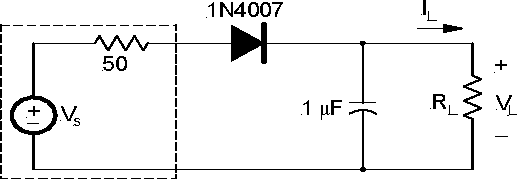
\includegraphics[width=\textwidth]{volt_rect}
%     \caption{\label{fig:volt_rect} Voltage rectifier circuit.}
%   \end{subfigure}%
%   ~
%   \begin{subfigure}[b]{0.4\textwidth}
%     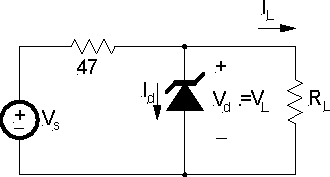
\includegraphics[width=\textwidth]{volt_reg}
%     \caption{\label{fig:volt_reg} Voltage regulator circuit.}
%   \end{subfigure}
%   \caption{\label{fig:circuits_tested} Circuits used in this lab.}
% \end{figure}

\section{Procedure}
\label{sec:procedure}

Prior to performing the lab, the Compact L298 Motor Driver Board was constructed in accordance with the directions included in the Kit.

\subsection{Part One}
\label{sec:part_one}

First, the ($+$) and ($-$) terminals of the motor driver board were connected to the \SI{6}{V} DC power supply via the breadboard.  Then the regulated \SI{+5}{V} (H) output of the motor driver board was connected to the breadboard, so it can be used in later steps to enable the driver logic.  Wires were connected to the motor output terminals on the left side of the motor driver board.  Inputs $L_1$, $L_2$, and $Enable$ (E1-2) were connected in accordance with Table~\ref{tab:logic}.  The output of the DC power supply was set to \SI{6}{V} and the motor output voltage ($V_{out}$) was measured and the LED lights were observed.  Results for each input configuration shown in Table~\ref{tab:logic} were also recorded in Table~\ref{tab:logic}.  Then, the output of the DC power supply was turned off and \SI{6}{V} DC motor was connected to the output of the motor driver board.  The output of the DC power supply was set to \SI{6}{V} and inputs were connected in accordance with Table~\ref{tab:logic} and the direction of motor rotation was also recorded in Table~\ref{tab:logic}.  Finally, $L_1$, $L_2$, and $Enable$ were set in the clockwise motor rotation (according to table 1)and the DC power supply was swept from \SI{6}{V} to \SI{3}{V} in \SI{0.1}{V} increments and the effects were observed.  The output of the DC power supply was turned off and DC motor was disconnected.

\subsection{Part Two}
\label{sec:part_two}

First the function generator was set to a square wave with a frequency of 20 kHz.  Channel 1 of the oscilloscope was connected to the output of the function generator and the square wave was offset for 0V to \SI{5}{V}.  $L_1$ and $L_2$ were again set for clockwise rotation and the $Enable$ input was connected to the function generator.  The DC power supply was turned on and set to \SI{6}{V}.  Then, the \%Duty of the square wave was swept from 20\% to 80\% in 10\% increments and the motor driver board output was recorded in Table~\ref{tab:duty}.  After that, the output of the DC power supply was turned off and the \%Duty of the function generator was rest to 50\%.  Then, the \SI{6}{V} DC motor was connected to the motor output of the motor driver board and the output of the DC power supply was set to \SI{6}{V}.  The \%Duty of the square wave was swept from 50\% to 80\% in 1\% increments and motor speed was observed.

\section{Results}
\label{sec:results}

\begin{table}[hbtp]
  \centering
  \begin{tabular}{ccc|ccc}
    Enable & \si{L_1} & \si{L_2} & \si{V_{out}} & LED & Motor \\
    \hline
    L & L & L & \SI{-0.01}{V} & off & off \\
    L & L & H & \SI{-0.01}{V} & off & off \\
    L & H & L & \SI{-0.01}{V} & off & off \\
    L & H & H & \SI{-0.01}{V} & off & off \\
    H & L & L & \SI{-0.18}{V} & off & off \\
    H & L & H & \SI{+5.7}{V} & red & CW \\
    H & H & L & \SI{+5.5}{V} & green & CCW \\
    H & H & H & \SI{+0.01}{V} & both & off \\
  \end{tabular}
  \caption{\label{tab:logic} Logic Table}
\end{table}

\begin{table}[hbtp]
  \centering
  \begin{tabular}{cc}
    Duty Cycle & \si{V_{out}} \\
    \hline
    20\% & \SI{-3.01}{V} \\
    30\% & \SI{-3.39}{V} \\
    40\% & \SI{-3.76}{V} \\
    50\% & \SI{-4.13}{V} \\
    60\% & \SI{-4.49}{V} \\
    70\% & \SI{-4.84}{V} \\
    80\% & \SI{-5.19}{V} \\
  \end{tabular}
  \caption{\label{tab:duty} Pulse-width modulation}
\end{table}

%\section{Comparison of Results}
%\label{sec:comp_of_res}

% The PSpice computed values of $V_{OC}$ shown in Table~\ref{tab:volt_reg_calc}, were very close to the measured $V_{OC}$ values (Table~\ref{tab:volt_reg_calc}), and were at most only 3.327\% different (Table~\ref{tab:volt_reg_diff}).  Also, the PSpice computed $V_S$ drop (Table~\ref{tab:volt_reg_calc}) was very close to the measured $V_S$ drop (Table~\ref{tab:volt_reg_meas}) and the percent difference was at most only 1.7\% (Table~\ref{tab:volt_reg_diff}).

\section{Conclusion}
\label{sec:conclusion}

The motor driver board can be adjusted to control the speed and direction of the DC motor through various mechanisms.  First, the $Enable$ input must ``see'' ~\SI{5}{V} before the Motor Drive Board can then allow the $L_1$ and $L_2$ inputs control the phase/rotation of the output.  To control the of the output voltage, the $L_1$ and $L_2$ inputs must also see ~\SI{5}{V} separately.  In our configuration, when $L_1$ was connected to \SI{5}{V}, the motor rotated counterclockwise (Table~\ref{tab:logic}).  When $L_2$ was connected, the motor turned clockwise (Table~\ref{tab:logic}). When both were connected or neither was connected, the motor didn't turn at all.

The motor driver board speed was adjusted via two different approaches in the experiment.  In part I, the input voltage was adjusted to proportionately affect the output voltage, thus varying the speed of the motor.  As input voltage was swept from high to low in part I, the motor speed slowed and eventually no noticeable turning could be observed at \SI{3}{V}.  In part II, the \%Duty of the \SI{5}{V} to the $Enable$ input was adjusted such that the time that \SI{5}{V} was seen at the $Enable$ input was varied from 50\% of the time to 80\% of the time which resulted in lower to higher Vrms accordingly.  This proportional change in \%Duty and output Vrms was observed and recorded Table~\ref{tab:duty}.

% \section{Equations}
% \label{sec:equations}

% % LaTeX sees blank lines as a start of another paragraph.  To avoid
% % unnecessary vertical spaces between equations, and still visually
% % separate in source, put a comment between them.
% %
% \begin{equation}
%   \label{eq:percent_diff}
%   \%_{diff} = \frac{|nominal - measured|}{nominal}\times 100\%
% \end{equation}
% %
% \begin{equation}
%   \label{eq:ripple}
%   V_r = V_{max} - V_{min}
% \end{equation}
% %
% \begin{equation}
%   \label{eq:volt_reg}
%   \%_{reg} = \frac{V_{load} - V_{no load}}{V_{no load}}\times 100\%
% \end{equation}

\end{document}
